

Facts about planet Mars\footnote{\url{https://en.wikipedia.org/wiki/Mars}}:
\begin{itemize}
\item average radius $R=3389.5 \pm 0.2 \si{\km}$
\item equatorial radius $3396.2 \pm 0.1 \si{\km}$
\item polar radius $3376.2 \pm 0.1 \si{\km}$
\item volume $1.6318 \cdot 10^{20} \si{\cubic\metre}$
\item mass $6.4171 \cdot 10^{23}\si{\kilo\gram}$
\item mean density $\langle\rho\rangle= 3934\si{\kilo\gram\per\cubic\meter}$
\item moment of inertia $I=0.3644 \pm 0.0005$
\item surface gravity $g=3.72076 \si{\metre\per\square\second}$
\end{itemize}

The surface gravity can be obtained with 
\[
g_{surf}=\frac{{\cal G} M}{R^2} 
=\frac{6.67430 \cdot 10^{-11} \; 6.4171 \cdot 10^{23} }{(3.3895\cdot 10^6)^2}
\simeq 3.727977
\]

The internal structure of the planet is not settled although 
it is now widely accepted that the planet has a core. 

B. Steinberger was kind enough to communicate to us the density and viscosity 
profiles used in Steinverger \etal (2010) \cite{stwt10} \footnote{Files sent to us 
we slightly altered for the purpose of this work. The density profile was missing 
the 50km near the center of the planet so padding was used. The viscosity profile 
starts below the moho at 50\si{\km} and stopped at the cmb. }:

\begin{center}
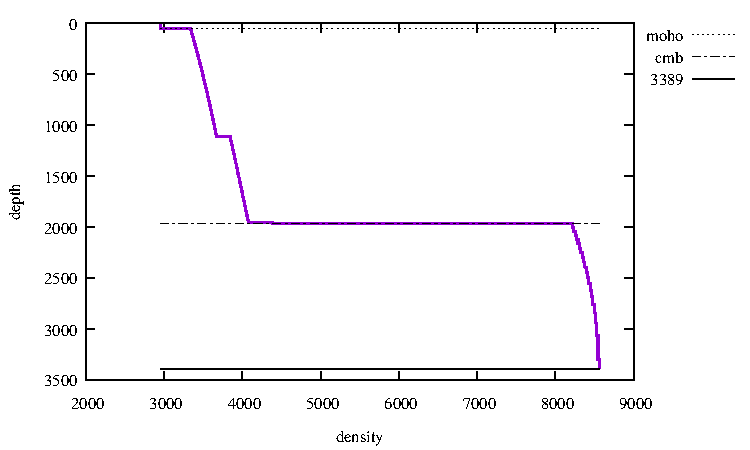
\includegraphics[width=7cm]{python_codes/fieldstone_96/data/rho1}
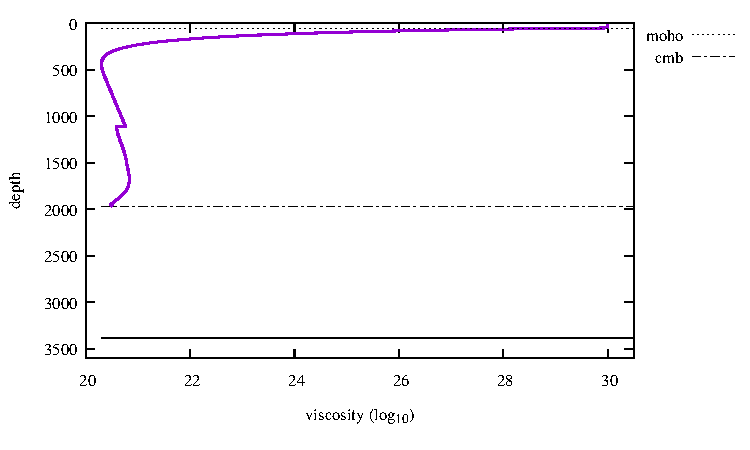
\includegraphics[width=7cm]{python_codes/fieldstone_96/data/eta1}\\
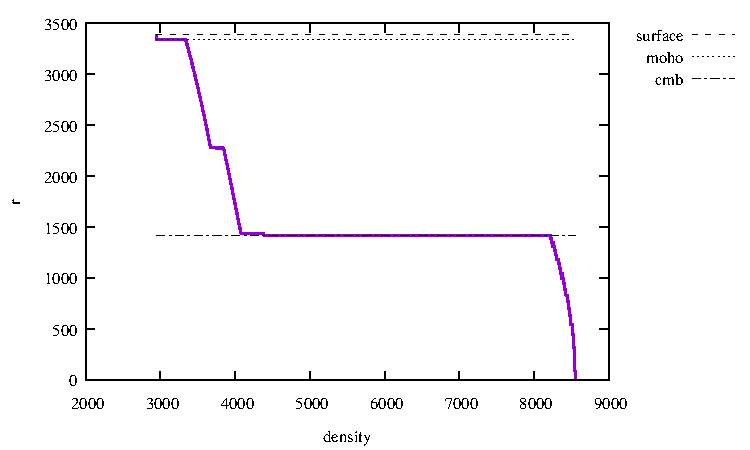
\includegraphics[width=7cm]{python_codes/fieldstone_96/data/rho2}
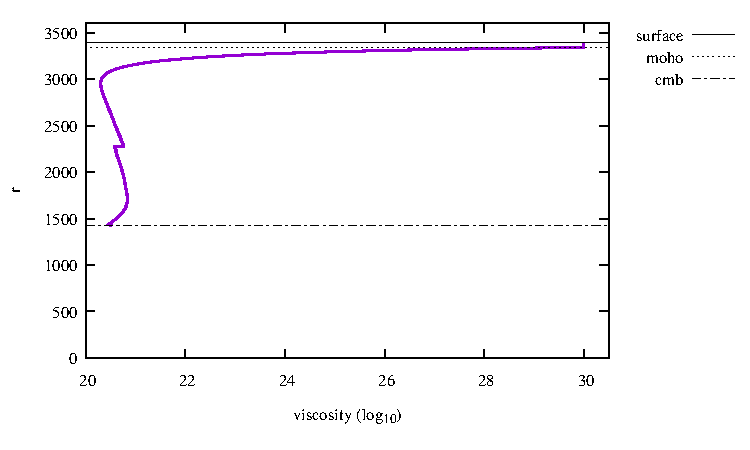
\includegraphics[width=7cm]{python_codes/fieldstone_96/data/eta2}\\
{\captionfont Data curtesy of B. Steinberger, from \cite{stwt10}} \\
{\tiny {\color{gray} in python\_codes/fieldstone\_96/data/}}
\end{center}


\begin{center}
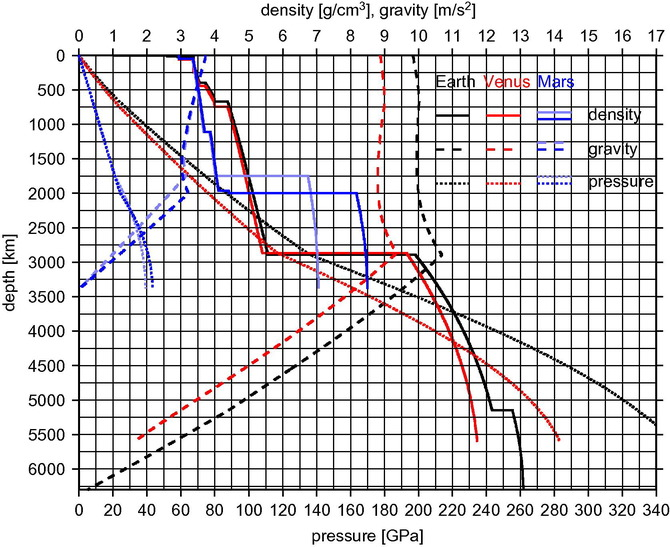
\includegraphics[width=5.7cm]{python_codes/fieldstone_96/images/stwt10_b}
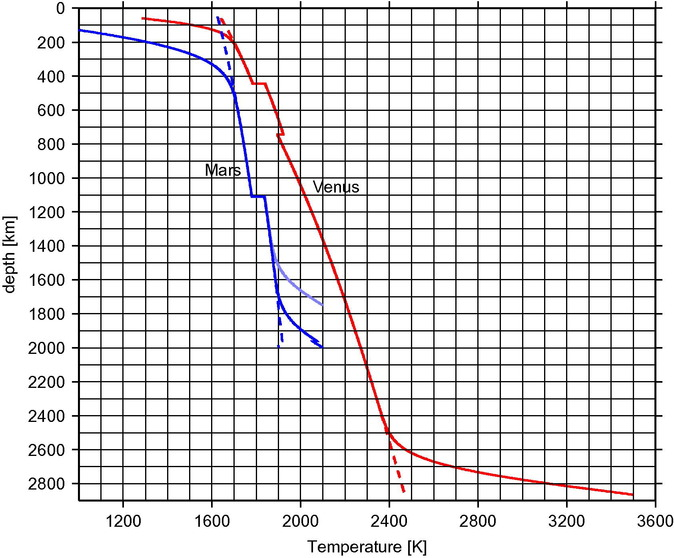
\includegraphics[width=5.7cm]{python_codes/fieldstone_96/images/stwt10_c}
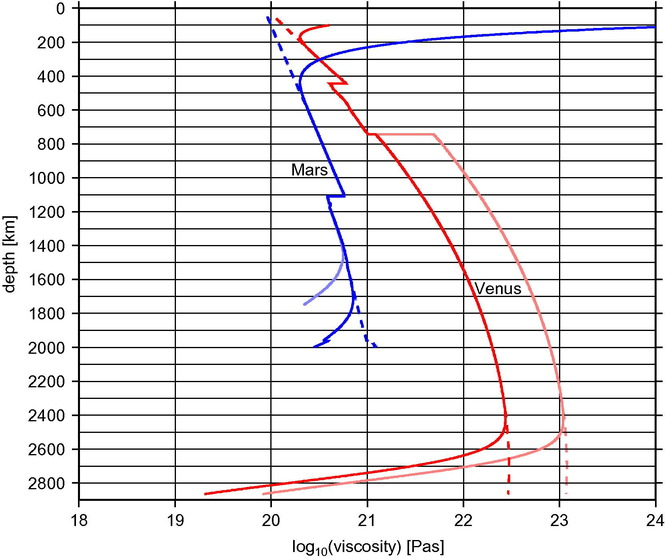
\includegraphics[width=5.7cm]{python_codes/fieldstone_96/images/stwt10_d}\\
{\captionfont Taken from Steinverger \etal (2010) \cite{stwt10}}
\end{center}

In table 1 of \cite{stwt10}: crust thickness is set to 50km. The core radius is set 
to 1389.5km. However in the data set we were sent it seems that the cmb is at 1422\si{\km}
radius.

To simplify things we take $R=3389\si{\km}$ and $R_{cmb}=1422\si{\km}$ in the code.
 
